\section{Сховішча даных}

\subsection{База даных}

Для захоўвання даных (інфармацыя пра жанры, аўтараў, кнігі, карыстальнікаў) выкарыстоўваецца
рэляцыйная база даных.

Рэляцыйная база даных --- гэта сукупнасць узаемазвязаных табліц, кожная з якіх утрымоўвае інфармацыю аб аб'ектах пэўнага тыпу. Радок табліцы змяшчае даныя аб адным аб'екце (напрыклад, кнігі, карыстальнікі), а слупкі табліцы апісваюць розныя характарыстыкі гэтых аб'ектаў --- атрыбутаў (напрыклад, логін карыстальніка, пароль карыстальніка). Запісы, г. зн. радкі табліцы, маюць аднолькавую структуру --- яны складаюцца з палёў, якія захоўваюць атрыбуты аб'екта. Кожнае поле, г. зн. слупок, апісвае толькі адну характарыстыку аб'екта і мае строга вызначаны тып даных. Усе запісы маюць адны і тыя ж палі, толькі ў іх адлюстроўваюцца розныя інфармацыйныя ўласцівасці аб'екта.

Для электроннай бібліятэкі была абраная рэляцыйная база даных MariaDB.

MariaDB Server --- адна з самых папулярных рэляцыйных баз даных з адкрытым зыходным кодам. Гэта зроблена арыгінальнымі распрацоўшчыкамі MySQL і гарантуецца, што застанецца праектам з адкрытым зыходным кодам.
MariaDB у наўнасці ў большасці воблачных рашэнняў і база даных па ўмаўчанні ў большасці дыстрыбутывах Linux.

MariaDB пабудавана на каштоўнасцях прадукцыйнасці, стабільнасці і адкрытасці. MariaDB Foundation гарантуе, што ўнёсак будзе прыняты па тэхнічных заслугах. Апошнія новыя функцыянальныя магчымасці ўключаюць у сябе пашыранае кластараванне з Galera Cluster 4, функцыі сумяшчальнасці з базай даных Oracle і часовымі табліцамі даных, што дазваляе запытаць даныя, якія яны былі ў любы момант мінулага.

Для спрашчэння разгортвання базы даных было вырашына карыстацца Amazon RDS сервісам (SaaS).

Amazon Relational Database Service (Amazon RDS) дазваляе проста наладжваць, выкарыстоўваць і маштабаваць рэляцыйныя базы даных у воблаку. Сeрвіс забяспечвае эканамічнае і маштабаванае выкарыстанне рэсурсаў пры адначасовай аўтаматызацыі працаёмкіх задач адміністравання, такіх як выдзяленне апаратнага забеспячэння, налада базы даных, ўстаноўка выпраўленняў і рэзервовае капіраванне. Гэта дазваляе засяродзіць увагу на праграмах, каб забяспечыць для іх высокую прадукцыйнасць, высокую даступнасць, бяспеку і сумяшчальнасць.

Amazon RDS даступны ў выглядзе машын базы даных некалькіх тыпаў: аптымізаваныя для працы з памяццю, для высокай прадукцыйнасці або выканання аперацый уводу-вываду --- і прапануе на выбар шэсць вядомых ядраў баз даных, у тым ліку Amazon Aurora, PostgreSQL, MySQL, MariaDB, Oracle Database і SQL Server. З дапамогай сeрвісу AWS Database Migration Service можна проста перанесці або рэпліцыраваць існуючыя базы даных у Amazon RDS.

\subsection{Amazon Simple Storage Service}

Так як рэляцыйныя базы даных не прызначаныя для захоўвання бінарных файлаў вялікіх памераў,
было вырашана ў базе даных захоўваць адрас (спасылку) на pdf файл, у той час як самі
pdf файлы захоўваць на асобным сервісе захоўвання аб'ектаў (Amazon S3).

Amazon Simple Storage Service (Amazon S3) --- гэта сeрвіс захоўвання аб'ектаў, які прапануе найлепшыя ў галінe паказчыкі прадукцыйнасці, маштабаванасці, даступнасці і бяспекі даных. Гэта азначае, што кліентам AWS могуць быць кампаніі любых памераў і з любых абласцей дзейнасці. Яны могуць выкарыстоўваць сeрвіс Amazon S3 для захоўвання і абароны любых аб'ёмаў даных у розных сітуацыях, напрыклад для забеспячэння працы сайтаў, мабільных прыкладанняў, для рэзервовага капіявання і аднаўлення, архівавання, карпаратыўных праграм, прылад IoT і аналізу вялікіх даных. Amazon S3 прапануе простыя ў выкарыстанні прылады адміністравання, якія дазваляюць арганізаваць даныя і сапраўды наладзіць абмежаванні доступу ў адпаведнасці патрэбам бізнесу або заканадаўчымі патрабаваннямі. Amazon S3 забяспечвае надзейнасць 99,999999999\% (11 дзявятак) і захоўвае даныя мільёнаў праграм у інтарэсах кампаній з усяго свету.

Перавагі Amazon S3:
\begin{enumerate}
    \item можна лёгка павялічваць і скарачаць рэсурсы сховішча ў адпаведнасці з ваганнямі патрэбаў, пры гэтым не патрабуюцца папярэднія ўкладанні або выдаткі на набыццё рэсурсаў. Сeрвіс Amazon S3 забяспечвае надзейнасць даных 99,999999999\% (11 дзявятак), паколькі ён аўтаматычна стварае і захоўвае копіі ўсіх аб'ектаў з S3 ў мностве незалежных сістэм. Гэта азначае, што даныя даступны, калі яны патрэбныя, і абаронены ад збояў, памылак і пагрозаў.
    \item магчымасць скарачаць выдаткі, не ахвяруючы прадукцыйнасцю, шляхам захоўвання даных у розных класах сховішчаў S3, якія забяспечваюць розныя ўзроўні доступу да даных па адпаведных расцэнках. Можна выкарыстоўваць аналіз класаў сховішчаў S3, каб выявіць даныя, якія варта перанесці ў менш затратны клас сховішча, на падставе мадэляў доступу да іх, а таксама наладзіць палітыку жыццёвага цыкла S3, каб выконваць перанос. Можна таксама захоўваць даныя ў мадэлях доступу , якія змяняюцца або невядомыя, у сістэме S3 Intelligent-Tiering, якая размяркоўвае аб'екты па ўзроўнях на падставе мадэляў доступу, якія змяняюцца, і аўтаматычна забяспечвае скарачэнне выдаткаў.
    \item абарона даных ад несанкцыянаванага доступу з дапамогай магчымасцяў шыфравання і інструментаў кіравання доступу. S3 --- гэта адзіны сeрвіс захоўвання аб'ектаў з магчымасцю блакавання публічнага доступу да ўсіх аб'ектаў у кошыку або на ўзроўні акаўнта з дапамогай функцыі S3 Block Public Access. S3 адпавядае нарматывам такіх стандартаў, як PCI-DSS, HIPAA/HITECH, FedRAMP, дырэктыва ЕЗ па абароне даных і FISMA, што дазваляе выканаць заканадаўчыя патрабаванні. AWS таксама падтрымлівае разнастайныя магчымасці аўдыту, каб адсочваць запыты на доступ да вашых рэсурсаў у S3.
\end{enumerate}

На малюнку \ref{img: DB graph} прадстаўлены граф сувязі базы даных, якая выкарыстоўваецца для вэб-сервера электронная бібліятэка.

\newpage

\begin{figure}[h!]
    \centering
    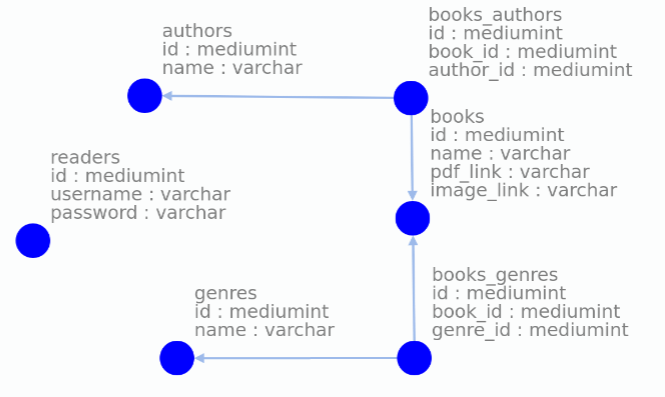
\includegraphics[width=\textwidth]{db_graph}
    \caption{Граф сувязі базы даных}
    \label{img: DB graph} 
\end{figure}

На малюнку \ref{img: DB graph} бачым, што база даных электроннай бібліятэкі складаецца з 6 табліц:
\begin{enumerate}
    \item authors:
    \begin{enumerate}
        \item id --- унікальны нумар запісу;
        \item name --- поўнае імя аўтара;
    \end{enumerate}
    \item books:
    \begin{enumerate}
        \item id --- унікальны нумар запісу;
        \item name --- назва кнігі;
        \item pdf\_link --- спасылка на pdf версію кнігі ў S3 кошыку;
        \item image\_link --- спасылка на вокладку кнігі ў S3 кошыку;
    \end{enumerate}
    \item genres:
    \begin{enumerate}
        \item id --- унікальны нумар запісу;
        \item name --- назва жанру;
    \end{enumerate}
    \item readers:
    \begin{enumerate}
        \item id --- унікальны нумар запісу;
        \item username --- імя карыстальніка для рэгістрацыі;
        \item password --- пароль карыстальніка для рэгістрацыі;
    \end{enumerate}
    \item books\_authors:
    \begin{enumerate}
        \item id --- унікальны нумар запісу;
        \item book\_id --- паказальнік на id кнігі ў табліцы books;
        \item author\_id --- паказальнік на id аўтара ў табліцы authors;
    \end{enumerate}

    \clearpage

    \item books\_genres:
    \begin{enumerate}
        \item id --- унікальны нумар запісу;
        \item book\_id --- паказальнік на id кнігі ў табліцы books;
        \item genre\_id --- паказальнік на id жанра ў табліцы genres;
    \end{enumerate}
\end{enumerate}

Можам заўважыць, што табліцы books, authors, genres, readers захоўваюць неабходную інфармацыю для
работы электроннай бібліятэкі, у той час як табліцы books\_authors і books\_genres выкарыстоўваюцца
для арганізацыі сувязі многія-многія паміж табліцамі ўнутры базы даных (пры дапамозе гэтых табліц
ажыццяўляецца злучэнне табліц ў аператары JOIN).

На малюнку \ref{img: DB example} прадстаўлены прыклад табліцы books.

\begin{figure}[h!]
    \centering
    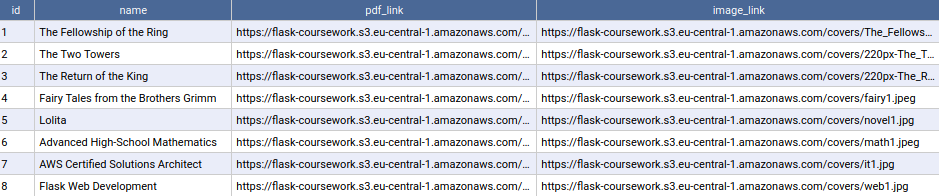
\includegraphics[width=\textwidth]{db_example}
    \caption{Прыклад табліцы books у базе даных}
    \label{img: DB example} 
\end{figure}
